% -*- Mode:TeX -*-

%% IMPORTANT: The official thesis specifications are available at:
%%            http://libraries.mit.edu/archives/thesis-specs/
%%
%%            Please verify your thesis' formatting and copyright
%%            assignment before submission.  If you notice any
%%            discrepancies between these templates and the 
%%            MIT Libraries' specs, please let us know
%%            by e-mailing thesis@mit.edu

%% The documentclass options along with the pagestyle can be used to generate
%% a technical report, a draft copy, or a regular thesis.  You may need to
%% re-specify the pagestyle after you \include  cover.tex.  For more
%% information, see the first few lines of mitthesis.cls. 

%\documentclass[12pt,vi,twoside]{mitthesis}
%%
%%  If you want your thesis copyright to you instead of MIT, use the
%%  ``vi'' option, as above.
%%
%\documentclass[12pt,twoside,leftblank]{mitthesis}
%%
%% If you want blank pages before new chapters to be labelled ``This
%% Page Intentionally Left Blank'', use the ``leftblank'' option, as
%% above. 

\documentclass[12pt,twoside,leftblank,draft]{upcthesis}
\usepackage{lgrind}
\usepackage{url}

% Cross reference between latex files
\usepackage{xr}
\externaldocument{chap1}
\externaldocument{chap2}
\externaldocument{chap3}
\externaldocument{chap4}
\externaldocument{chap5}

% Minted color style
\usemintedstyle{github}

%% This bit allows you to either specify only the files which you wish to
%% process, or `all' to process all files which you \include.
%% Krishna Sethuraman (1990).

%%\typein [\files]{Enter file names to process, (chap1,chap2 ...), or `all' to process all files:}
%%\files{all}
\def\all{all}
%%\ifx\files\all \typeout{Including all files.} \else \typeout{Including only \files.} \includeonly{\files} \fi

\begin{document}

% -*-latex-*-
% 
% For questions, comments, concerns or complaints:
% thesis@mit.edu
% 
%
% $Log: cover.tex,v $
% Revision 1.8  2008/05/13 15:02:15  jdreed
% Degree month is June, not May.  Added note about prevdegrees.
% Arthur Smith's title updated
%
% Revision 1.7  2001/02/08 18:53:16  boojum
% changed some \newpages to \cleardoublepages
%
% Revision 1.6  1999/10/21 14:49:31  boojum
% changed comment referring to documentstyle
%
% Revision 1.5  1999/10/21 14:39:04  boojum
% *** empty log message ***
%
% Revision 1.4  1997/04/18  17:54:10  othomas
% added page numbers on abstract and cover, and made 1 abstract
% page the default rather than 2.  (anne hunter tells me this
% is the new institute standard.)
%
% Revision 1.4  1997/04/18  17:54:10  othomas
% added page numbers on abstract and cover, and made 1 abstract
% page the default rather than 2.  (anne hunter tells me this
% is the new institute standard.)
%
% Revision 1.3  93/05/17  17:06:29  starflt
% Added acknowledgements section (suggested by tompalka)
% 
% Revision 1.2  92/04/22  13:13:13  epeisach
% Fixes for 1991 course 6 requirements
% Phrase "and to grant others the right to do so" has been added to 
% permission clause
% Second copy of abstract is not counted as separate pages so numbering works
% out
% 
% Revision 1.1  92/04/22  13:08:20  epeisach

% NOTE:
% These templates make an effort to conform to the MIT Thesis specifications,
% however the specifications can change.  We recommend that you verify the
% layout of your title page with your thesis advisor and/or the MIT 
% Libraries before printing your final copy.
\title{Renewable Energy Production Distribution Map of
Catalan Homes}

\author{Pau P\'{e}rez Fabregat}
% If you wish to list your previous degrees on the cover page, use the 
% previous degrees command:
%       \prevdegrees{A.A., Harvard University (1985)}
% You can use the \\ command to list multiple previous degrees
%       \prevdegrees{B.S., University of California (1978) \\
%                    S.M., Massachusetts Institute of Technology (1981)}
\department{Department of Service and Information System Engineering}

% If the thesis is for two degrees simultaneously, list them both
% separated by \and like this:
% \degree{Doctor of Philosophy \and Master of Science}
\degree{Informatics Engineering}

% As of the 2007-08 academic year, valid degree months are September, 
% February, or June.  The default is June.
\degreemonth{February}
\degreeyear{2014}
\thesisdate{Jan 10, 2014}

% If there is more than one supervisor, use the \supervisor command
% once for each.
\supervisor{Carles Farr\'{e} Tost}{Associate Professor}

% This is the department committee chairman, not the thesis committee
% chairman.  You should replace this with your Department's Committee
% Chairman.
\chairman{Carles Farr\'{e} Tost}{Chairman}

% Make the titlepage based on the above information.  If you need
% something special and can't use the standard form, you can specify
% the exact text of the titlepage yourself.  Put it in a titlepage
% environment and leave blank lines where you want vertical space.
% The spaces will be adjusted to fill the entire page.  The dotted
% lines for the signatures are made with the \signature command.
\maketitle

% The abstractpage environment sets up everything on the page except
% the text itself.  The title and other header material are put at the
% top of the page, and the supervisors are listed at the bottom.  A
% new page is begun both before and after.  Of course, an abstract may
% be more than one page itself.  If you need more control over the
% format of the page, you can use the abstract environment, which puts
% the word "Abstract" at the beginning and single spaces its text.

%% You can either \input (*not* \include) your abstract file, or you can put
%% the text of the abstract directly between the \begin{abstractpage} and
%% \end{abstractpage} commands.

% First copy: start a new page, and save the page number.
\cleardoublepage
% Uncomment the next line if you do NOT want a page number on your
% abstract and acknowledgments pages.
% \pagestyle{empty}
\setcounter{savepage}{\thepage}
\begin{abstractpage}
% $Log: abstract.tex,v $
% Revision 1.1  93/05/14  14:56:25  starflt
% Initial revision
% 
% Revision 1.1  90/05/04  10:41:01  lwvanels
% Initial revision
% 
%
%% The text of your abstract and nothing else (other than comments) goes here.
%% It will be single-spaced and the rest of the text that is supposed to go on
%% the abstract page will be generated by the abstractpage environment.  This
%% file should be \input (not \include 'd) from cover.tex.
In this thesis...

\end{abstractpage}

% Additional copy: start a new page, and reset the page number.  This way,
% the second copy of the abstract is not counted as separate pages.
% Uncomment the next 6 lines if you need two copies of the abstract
% page.
% \setcounter{page}{\thesavepage}
% \begin{abstractpage}
% % $Log: abstract.tex,v $
% Revision 1.1  93/05/14  14:56:25  starflt
% Initial revision
% 
% Revision 1.1  90/05/04  10:41:01  lwvanels
% Initial revision
% 
%
%% The text of your abstract and nothing else (other than comments) goes here.
%% It will be single-spaced and the rest of the text that is supposed to go on
%% the abstract page will be generated by the abstractpage environment.  This
%% file should be \input (not \include 'd) from cover.tex.
In this thesis...

% \end{abstractpage}

\cleardoublepage

\section*{Acknowledgments}

This is the acknowledgements section.  You should replace this with your
own acknowledgements.

%%%%%%%%%%%%%%%%%%%%%%%%%%%%%%%%%%%%%%%%%%%%%%%%%%%%%%%%%%%%%%%%%%%%%%
% -*-latex-*-

% Some departments (e.g. 5) require an additional signature page.  See
% signature.tex for more information and uncomment the following line if
% applicable.
% % -*- Mode:TeX -*-
%
% Some departments (e.g. Chemistry) require an additional cover page
% with signatures of the thesis committee.  Please check with your
% thesis advisor or other appropriate person to determine if such a 
% page is required for your thesis.  
%
% If you choose not to use the "titlepage" environment, a \newpage
% commands, and several \vspace{\fill} commands may be necessary to
% achieve the required spacing.  The \signature command is defined in
% the "mitthesis" class
%
% The following sample appears courtesy of Ben Kaduk <kaduk@mit.edu> and
% was used in his June 2012 doctoral thesis in Chemistry. 

\begin{titlepage}
\begin{large}
This doctoral thesis has been examined by a Committee of the Department
of Chemistry as follows:

\signature{Professor Jianshu Cao}{Chairman, Thesis Committee \\
   Professor of Chemistry}

\signature{Professor Troy Van Voorhis}{Thesis Supervisor \\
   Associate Professor of Chemistry}

\signature{Professor Robert W. Field}{Member, Thesis Committee \\
   Haslam and Dewey Professor of Chemistry}
\end{large}
\end{titlepage}


\pagestyle{drafthead}
  % -*- Mode:TeX -*-
%% This file simply contains the commands that actually generate the table of
%% contents and lists of figures and tables.  You can omit any or all of
%% these files by simply taking out the appropriate command.  For more
%% information on these files, see appendix C.3.3 of the LaTeX manual. 
\tableofcontents


%% This is an example first chapter.  You should put chapter/appendix that you
%% write into a separate file, and add a line \include{yourfilename} to
%% main.tex, where `yourfilename.tex' is the name of the chapter/appendix file.
%% You can process specific files by typing their names in at the 
%% \files=
%% prompt when you run the file main.tex through LaTeX.
\chapter{Introduction}

The Center for Ecological Research and Forestry Applications (CREAF) is a public research institution that was created in 1987.  The members of the Governing Council of CREAF are the Generalitat of Catalonia, the Autonomous University of Barcelona (UAB), University of Barcelona (UB), the Institute for Research and Technology (IRTA), the Institute of Catalan Studies (IEC) and the Spanish National Research Council (CSIC).

Its objective is to generate knowledge and create new methodological tools in the field of terrestrial ecology, with special emphasis on forest ecology, in order to improve environmental planning and management in rural and urban areas. This is achieved, among other means, through the development of methodological and conceptual tools designed to facilitate decision-making and improve environmental management.

Since its creation, CREAF has made very important contributions to the field of terrestrial ecology and towards a sustainable management of the environment. This has been achieved through research, development, training and technology transfer. Some of its outstanding breakthroughs are the design and implementation of the Ecological and Forest Inventory of Catalonia (EFIC), innovative at the international level due to the incorporation of new ecological parameters, the production of the Land Cover Map of Catalonia (MCSC), a high-resolution digital map for environmental assessment and territorial planning and management and the development of the MiraMon \copyright  Geographic Information System, widely adopted in Catalan administration and currently being used in over thirty countries around the world.


\section{Motivations}

The motivation for this master thesis arise from the idea that the wide development of web technology such as HTML5, PaaS, IaaS, NoSQL and the steady increase in Open Source adoption in recent years make possible the implementation of powerful systems with significant cuts on budget. Moreover these technologies often come with (entail?) considerable improvements in maintainability, performance and reduced complexity.

I am firmly convinced that this set of technologies and tools could improve research in centres such as CREAF, providing them with better and affordable infrastructures that allow to reduce the timespan of common processes and calculations. Moreover, they provide new means for the dissemination of the valuable data that result from these processes.

I think that computer engineering should be conceived as a tool to push forward the development of other sciences. In particular, as recently graduated engineers we can contribute with our acquired knowledge to the society attempting to solve problems that benefit us all. Therefore, I wish to develop a project whose outcome could improve the work of some public research centre becoming a useful tool.

Given my discovered interest in topics like distributed computing, sensor networks and resilience systems arouse in my recent stay in University of Antwerp I am eager for expanding my knowledge farther and dig deeper into these fields relating them in a real-world use case.

Within in the context of volunteered geographic information (VGI) and renewable energies CREAF wants to solve the problem of knowing the distribution of renewable energy produced in Catalan homes. Nowadays the actual distribution of the energy produced by either wind or solar systems and their performance and evolution over time are unknown complicating the decision-making process regarding renewable energies in Catalonia.

On the other hand, CREAF wishes to expand its methodological tools by adopting sensor web. The reduced cost of hardware devices like Raspberry Pi and Arduino  and their general-purpose features make them an affordable option as sensor devices and facilitates the development of sensor client software. For these reasons, CREAF aims to deploy its own sensor devices in wild nature in the near future. 

Although some points were already clear, some others such as the architecture of the whole system to which the sensor clients will connect to as well as the software they would be shipped with were unknown for CREAF.

\section{Project Goals}

This project is aimed to develop a system that offers features to registered users’, those who freely share their data, and some other features available for all internet users. It will visualize the energy production of the clients’ system and its contribution to the whole Catalan renewable energy production in a real time map, while offering a private analytics dashboard to registered users where they can figure out the actual performance of their system.

Given the extent of the desired product we will develop a proof of concept; a distributed computing based system containing base features being a simple yet functional prototype of the final product. Once built the system results and metrics will be evaluated and its architecture may eventually become the standard infrastructure basis for future CREAF projects that demand sensor data.

Hence, the private features for registered users are out of the scope. TODO extend to clearly specify what is going to be out of the scope

TODO cite that the sensor devices are going to be either Raspberry Pi or Arduino

Hence, these two general goals are translated to the following specific goals (describe further the fact that we have a reduced scope; we don't have time for all):

\begin{itemize}
	\item Provide a command line interface that allows the simulation of the sensors functionality
	\item Develop a functional system that stores and processes the sensor observations
	\item Implement a simple public web application to show the real time data
\end{itemize}

\section{Methodolgy}

\subsection{Iterative Development}
Although advocating for agile software methodologies the concept-proof nature of the project and the fact that it's currently developed by just one person make them an unsuitable choice. We vote for a custom adaptation of iterative development, instead.

In conjunction with incremental development Iterative development is a way of breaking down the development of a software system in smaller chunks and repeated cycles. In each cycle, referred to as iteration, the slice of functionality is designed, developed, tested, deployed and evaluated. This allows software developers to apply the knowledge acquired in previous iterations, so the first implementation whose goal is to build a bare minimal functional system is iteratively enhanced so as to meet the requirements.

Nevertheless, iterative and incremental development are the basis for Agile development. Therefore, by adhering to these basis we attempt to avoid the agile practices and constraints that may be pointless in this case. Doing so, we aim to progressively enhance the codebase in subsequent iterations, gain insight into the architecture and improve any weak points we may identify until eventually meeting the requirements. Additionaly, by this way early results can be achieved and evaluated by CREAF resulting in a smoother collaboration.

\subsection{Test-Driven Development}

The chosen methodology also includes Test-Driven Development, which is a developer practice that involves writing tests before writing the code being tested. The initially failing test defines the behaviour of the code to be written, then the developer writes the minimum amount of code required to pass the test. Once it passes, it is time for refactoring the resulting design to remove any duplication. To further extend the responsibilities of the code this cycle must be repeated as many times as it requires.

Besides validating the correctness of the code, by driving the design of the program in small chunks through test cases the developer is mainly concerned with the interface of the program rather than its actual implementation.

What we aim for while using TDD in this project is to obtain a more modularized, maintainable, and extensible code. The development of the software in small units leads to smaller, more focused and loosely coupled classes and cleaner interfaces. The main benefit we may get by this means, however, is the greater level of confidence in the code caused by the fact that all written covered by at least one test.

Additionally, in this early stage of the project is basic for the successful evolution of the project to have a test-covered code. So it can be ensured that it keeps its intended behaviour and any defects are caught early in the development process.

TODO: NOTE ON THE LATTER CHAPTER THAT BY FOCUSING ON BEHAVIOUR TESTS FIRST WE GET A EXECUTABLE SPECIFICATION, SPECIALLY WITH RSPEC. BUT "TESTS ARE NOT A REPLACEMENT FOR SPECIFICATION" http://www.eiffel.com/general/column/2004/september.html. LEADS TO A LESS FORMAL SPECIFICATION.
TODO: REFERENCE http://agilepainrelief.com/notesfromatooluser/2008/10/advantages-of-tdd.html
TODO: CITE Madeyski, L. "Test-Driven Development - An Empirical Evaluation of Agile Practice"
%% This is an example first chapter.  You should put chapter/appendix that you
%% write into a separate file, and add a line \include{yourfilename} to
%% main.tex, where `yourfilename.tex' is the name of the chapter/appendix file.
%% You can process specific files by typing their names in at the 
%% \files=
%% prompt when you run the file main.tex through LaTeX.
\chapter{Analysis}

\section{Requirements}
They have been obtained throughout some interviews with the CREAF researcher in charge of the project.

Real use-case data (number of owners) has been obtained to "scope" the system qualities properly.

\subsection{System-Wide Functional Requirements}

\begin{itemize}
	\item The system must be fed with the data collected by the sensor devices
	\item The system must require an authentication system for the sensor devices and the web application users
	\item The system must provide software tracing
\end{itemize}

\subsubsection{System Qualities}

\subsubsection{Usability}

\begin{itemize}
	\item The system must be user friendly and easy to use by means of a GUI
	\item The sensor devices must be easy to set up by end users
	\item The sensor device must collect and deliver the data automatically
	\item All the command line interfaces must be scriptable and configurable
\end{itemize}

\subsubsection{Reliability}

\begin{itemize}
	\item The system must be reliable in low bandwidth and high network latency
	\item The system must be reliable in high-load scenarios
	\item The system must be reliable in high user concurrency scenarios
\end{itemize}

\subsubsection{Performance}

\begin{itemize}
	\item The sensor devices must be able to send [Y] request per hour
	\item The system must be able to process observations received from [X] sensor devices
	\item The system must able to show new available data in the real time visualization before the next observation is sent from the sensor device
\end{itemize}

\subsubsection{Supportability}

\begin{itemize}
	\item The system must have an event logging system
	\item The system must support SOS standard in order to be interoperable
	\item The system must be horizontally scalable
	\item The codebase must be maintainable and extendible
\end{itemize}

\subsection{System Interfaces}

\subsubsection{Interfaces to External Systems}

\begin{itemize}
	\item The system must integrate 52 North SOS implementation to provide a standard interoperability layer
\end{itemize}

\subsection{System Constraints}

\begin{itemize}
	\item The sensor devices must send [X] power observations within an hour
	\item The system must be able to run in commodity servers 
	\item The software must be portable in order to be deployed in any platform including PaaS and IaaS
\end{itemize}

SOS

\subsection{System Compliance}

\begin{itemize}
	\item The system and all its components must adhere to [Open Source license] license
\end{itemize}


\section{Technology Research}

%% This is an example first chapter.  You should put chapter/appendix that you
%% write into a separate file, and add a line \include{yourfilename} to
%% main.tex, where `yourfilename.tex' is the name of the chapter/appendix file.
%% You can process specific files by typing their names in at the 
%% \files=
%% prompt when you run the file main.tex through LaTeX.
\chapter{Specification}

The following section describes what the system does by detailing its entities.

\section{Use Case Model}

This section describes the operations of the systems as events triggered by external actors and their interrelation.

\subsection{Actors} \label{actors}

The actors of the system are the following.

\begin{description}
	\item[Sensor device] The device responsible for registering itself in the system and sending the measured observations to it.
	\item[User] A person who interacts with the public web application that shows the observations in a data visualization.
\end{description}

\subsection{Use Cases}

\begin{figure}[ht]
	\centering
	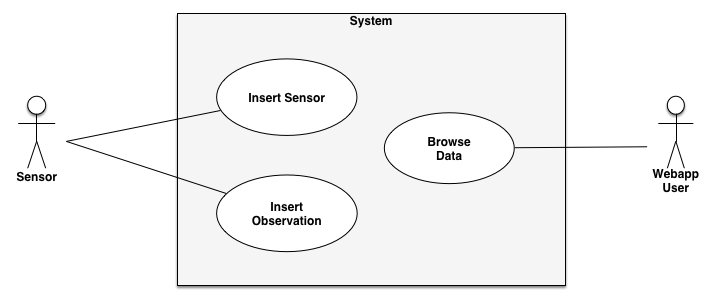
\includegraphics[width=\textwidth]{uses_cases}
	\caption{System use cases}
	\label{fig:use_cases}
\end{figure}

\begin{usecase}
	\addtitle{Use Case 1}{Insert Sensor}
	\addfield{Actors:}{Sensor device}
	\addfield{Preconditions:}{The system is running}
	\addfield{Postconditions:}{The sensor is registered and persisted in the system}
	\addscenario{Main Success Scenario:}{
		\item The sensor sends a request to register itself
		\item The system stores the information of the sensor in the database
		\item The system notifies the sensor when it has been successfully registered
	}
	\addscenario{Extensions:}{
		\item[1.a] The sensor is already registered
			\begin{enumerate}
			\item[1.] The system returns an error response
			\end{enumerate}
	}
\end{usecase}

\begin{usecase}
	\addtitle{Use Case 2}{Insert Observation}
	\addfield{Actors:}{Sensor device}
	\additemizedfield{Preconditions:}{
		\item The system is running
		\item The sensor is registered in the system	
	}
	\additemizedfield{Postconditions:}{
		\item The observation is persisted in the system
		\item The observation is sent to the web application tier
	}
	\addscenario{Main Success Scenario:}{
		\item The sensor sends a request to store the observation
		\item The system stores the observation data in the database
		\item The system sends the observation data to the web application tier
		\item The system notifies the sensor when the observation has been successfully stored
	}
	\addscenario{Extensions:}{
		\item[1.a] The sensor specified in the request is not found
			\begin{enumerate}
			\item[1.] The system returns an error message
			\end{enumerate}
	}
\end{usecase}

\begin{usecase}
	\addtitle{Use Case 3}{Browse data}
	\addfield{Actors:}{User}
	\addfield{Preconditions:}{The system is running}
	\addfield{Postconditions:}{The web application is shown}
	\addscenario{Main Success Scenario:}{
		\item The user's browser loads the web application
		\item Once loaded, the web application establishes a connection against the system
		\item The system incorporates observations into the web application as they are available
	}
\end{usecase}

\section{Conceptual Model}

As shown in figure \ref{fig:use_cases}, the system revolves around the concepts of \textit{Observation} and \textit{Sensor}. Diagram \ref{fig:conceptual_model} describes these concepts and other entities involved in the system as well as their relations, heavily based on the OGC O\&M model \cite{OM}.

To start with, an observation is an aggregation of the following six elements:

\begin{description}
\item[Feature of interest] A representation of a real-world object that carries the observed property, e.g. "Pant\`a de Sau". Hence, for an in-place instrument this would be the sensor location, whereas for a remote sensor it would be the target location.
\item[Procedure] Instance of a process which has performed the observation. Despite being usually a physical sensor, it can also be a process that leads to an observation such as a computation or the result of post-processing.
\item[Observed property] Represent the phenomena under observation. Usually a concept of a formal ontology, e.g. air temperature.
\item[Phenomenon time] Time when the phenomenon that produces the observation occurs.
\item[Result time] Time when the observation result has been created. Note that phenomenon and result times may be identical.
\item[Result] Result of the observation, which can be either a scalar value or a complex multi-dimensional array.
\end{description}

\begin{figure}[h]
	\centering
	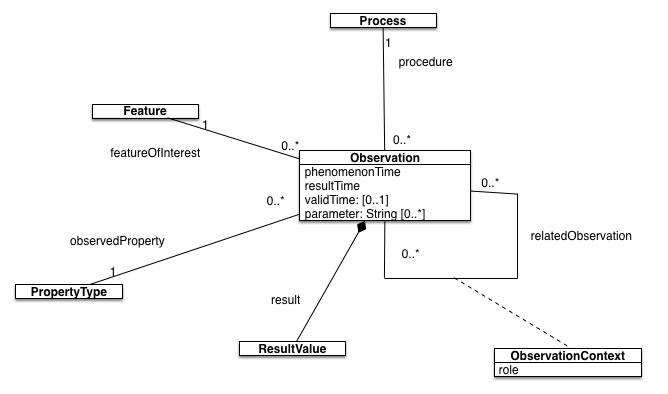
\includegraphics[width=\textwidth]{conceptual_model}
	\caption{Conceptual model}
	\label{fig:conceptual_model}
\end{figure}
\newpage

\section{Sequence Diagrams}

\begin{figure}[ht]
	\centering
	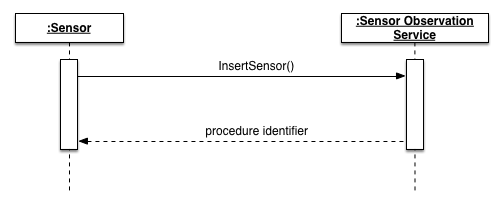
\includegraphics[scale=.75]{insert_sensor_seq}
	\caption{Sequence Diagram - Insert Sensor}
	\label{fig:insert_sensor_seq}
\end{figure}

\begin{figure}[ht]
	\centering
	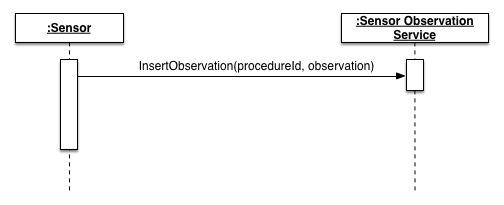
\includegraphics[scale=.75]{insert_observation_seq}
	\caption{Sequence Diagram - Insert Observation}
	\label{fig:insert_observation_seq}
\end{figure}

\begin{figure}[ht]
	\centering
	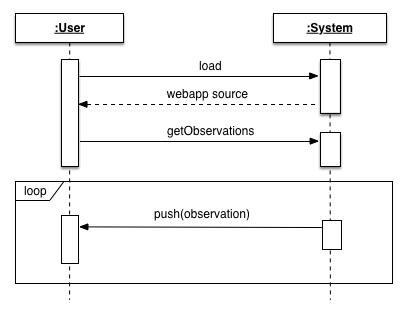
\includegraphics[scale=.75]{browse_data_seq}
	\caption{Sequence Diagram - Browse Data}
	\label{fig:browse_data_seq}
\end{figure}

%% This is an example first chapter.  You should put chapter/appendix that you
%% write into a separate file, and add a line \include{yourfilename} to
%% main.tex, where `yourfilename.tex' is the name of the chapter/appendix file.
%% You can process specific files by typing their names in at the 
%% \files=
%% prompt when you run the file main.tex through LaTeX.
\chapter{Specification}

The following section describes what the system does detailing its features.

\section{Uses Case Model}

This section describes the services of the systems as events triggered by external actors and their interrelation.

\subsection*{Actors}

The actors of the system are:

\begin{description}
	\item[Sensor device] The device responsible for registering itself in the system and sending the gathered observations to it. As the design and building of the sensor device is out of the scope of the project, it is simulated by a CLI tool that allows to issue request against the system.
	\item[Web application user] A person who interacts with the public web application that shows the observations in a data visualization.
\end{description}

\subsection{Use Cases}

\begin{figure}[h]
	\centering
	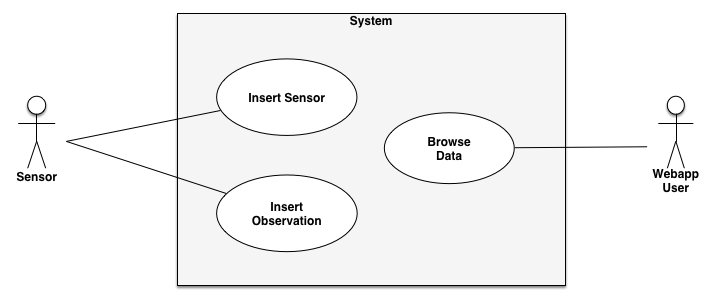
\includegraphics[width=\textwidth]{uses_cases}
	\caption{System's use cases}
	\label{fig:use_cases}
\end{figure}

\begin{usecase}
	\addtitle{Use Case 1}{Insert Sensor}
	\addfield{Actors:}{Sensor device}
	\addfield{Preconditions:}{The system is running}
	\addfield{Postconditions:}{The sensor is registered and persisted in the system}
	\addscenario{Main Success Scenario:}{
		\item The sensor issues a POST request to the sensors endpoint
		\item The system stores the sensor's information in the database
		\item The system sends a HTTP response with 201 status code to the sensor
	}
\end{usecase}

\begin{usecase}
	\addtitle{Use Case 2}{Insert Observation}
	\addfield{Actors:}{Sensor device}
	\additemizedfield{Preconditions:}{
		\item The system is running
		\item The sensor is registered in the system	
	}
	\additemizedfield{Postconditions:}{
		\item The observation is persisted in the system
		\item The observation is sent to the web application tier
	}
	\addscenario{Main Success Scenario:}{
		\item The sensor issues a POST request to the observations endpoint
		\item The system stores the observation's data in the database
		\item The system sends the observation's data to the web application tier
		\item The system sends a HTTP response with 201 status code to the sensor
	}
\end{usecase}

\section{Conceptual Model}

%% This is an example first chapter.  You should put chapter/appendix that you
%% write into a separate file, and add a line \include{yourfilename} to
%% main.tex, where `yourfilename.tex' is the name of the chapter/appendix file.
%% You can process specific files by typing their names in at the 
%% \files=
%% prompt when you run the file main.tex through LaTeX.
\chapter{Design}

In this chapter we will discuss all design decisions taken regarding the building of REDCH. These are grounded on the detailed research explained in Chapter \ref{technology_research}. The high-level architecture already outlined in \ref{fig:use_cases} is extended further by first explaining the technology used: the programming languages, frameworks and most relevant libraries. Then, the whole architecture of the system is presented by describing each one of the components the system is comprised of.

The design explained below aims to provide a solid groundwork and a first prototype for the REDCH project. Therefore, not all ideas discussed in previous chapters may be included in the result of this master thesis.

Ruby has been chosen as the main language for the development of the project. This dynamic language focused on simplicity and productivity is often regarded as developer performant. Due to its flexibility and similarity with natural language along with the massive amount of libraries and frameworks available, it allows developers to write applications very quickly. However, these features may hamper its execution performance.

\section{Physical Architecture}

The core idea of this architecture is to decouple the data producers from the data consumers by means of an asynchronous message queue enabling push capabilities in the consumption tier. It is compound of four different servers, as shown in figure \ref{fig:physical_architecture}: an application server that receives the observations from the sensors and stores them in the database. That server is also responsible for publishing them into the messaging queue. Then the messaging queue makes them available to the data consumption tier, where the app server sends them to the web clients.

\begin{figure}[H]
	\centering
	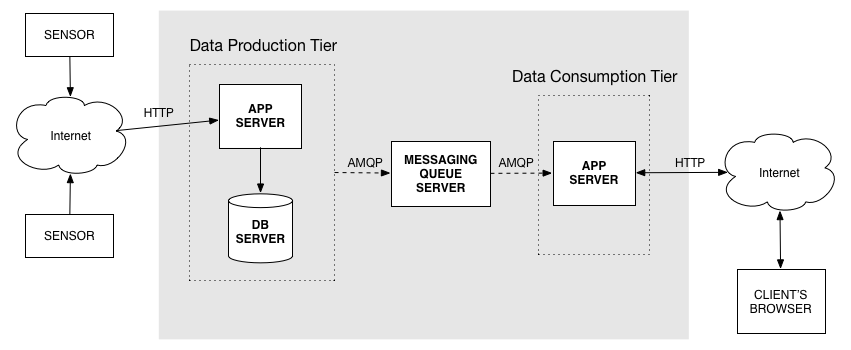
\includegraphics[width=\textwidth]{physical_architecture}
	\caption{Physical Architecture}
	\label{fig:physical_architecture}
\end{figure}

Such architecture brings about a number of benefits, as outlined in \ref{technology_research}. First and foremost, each tier can easily scale out independently. In both tiers, high availability and increased throughput can be provided through redundancy \cite{UA:resilience}, that is, adding more app servers. As for the database and the messaging queue, clusterizing them can provide better performance, increased throughput and storage capacity.

The loosely coupled architecture that the messaging queue provides along with the benefits stated in \ref{message_passing}, not only enables horizontally scaling but also allows components to evolve independently. The only constraint is that both tiers must understand the Advanced Message Queuing Protocol (AMQP). On the other hand, given the wide adoption of such protocol, the particular messaging queue may be replaced without affecting any of the tiers.

Finally, a high-performance asynchronous messaging queue provides real-time capabilities to the system.

\section{Logical Architecture}

\subsection{Sensor}

As already stated in \ref{actors}, although we opt for a solution that may involve RaspberryPi, the development of the sensor device falls beyond the scope of this project. Nonetheless, the system requires some sort of client in order to simulate its functioning in normal conditions.

\begin{figure}[h]
\centering
\begin{minipage}{.45\textwidth}
	\centering
	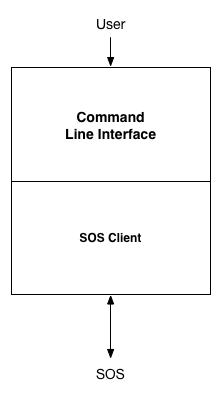
\includegraphics[width=.65\textwidth]{sensor_logic_view}
	\caption{Simulator Logic View}
	\label{fig:sensor_logic_view}
\end{minipage}
\begin{minipage}{.45\textwidth}
	\centering
	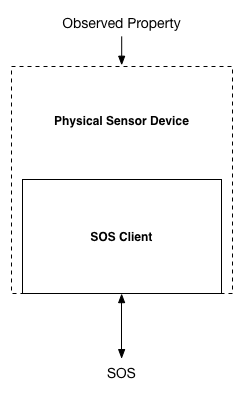
\includegraphics[width=.65\textwidth]{future_sensor_logic_view}
	\caption{Sensor Logic View}
	\label{fig:future_sensor_logic_view}
\end{minipage}
\end{figure}

A CLI acts as a presentation layer that enables interaction with the underlying SOS API client thus allowing the particular features of the sensor to be simulated. This approach offers the advantage of reusing the SOS client as a component of the final sensor device.

\subsubsection*{Command Line Interface}

On one hand, the \texttt{Redch} global namespace comprehends the CLI's commands. Similar to the command pattern, each class is named after the command it enables and contains all the logic for that particular command. As \ref{fig:cli_class_diagram} shows, the \texttt{Redch::CLI} class itself is a Thor application that exposes its interface in the command line, receives the input, executes the commands and prints their output.

Thor is a toolkit for building powerful command-line interfaces, which is used by well-known frameworks and tools such as Bundler, Ruby on Rails or Vagrant. The Thor class exposes a command-suite command-line application like Git that leads to very polished and easy-to-maintain command-line applications. In any Thor subclass, public methods become commands. Furthermore, Thor provides an interface to easily specify options and flags as a command's metadata, along with methods to specify the description of the commands. These are then included in a automatically generated \texttt{help} command.

\subsubsection*{Sensor Observation Service Client}

On the other hand, each command calls the underlying SOS Client, which in turn makes an HTTP request to the service. Being SOS a RESTful Web Service, the client implements two REST resources: \texttt{sensors} and \texttt{observations}, using the Ruby's rest-client gem\footnote{Libraries in Ruby programming language}.

This widely-used gem abstracts the actual HTTP protocol by exposing methods for each HTTP verb that accept header and query parameters to be passed in. Additionally, it provides a lower-level API that enables specification OF SSL parameters, dealing with cookies, etc. for cases the general API doesn't cover.

Finally, the client uses the Slim template language to render Geography Markup Language (GML), an OGC standard adopted by the International Organization for Standardization (ISO). Each operation has its own template that gets rendered with the data provided by each call. The obtained XML markup makes up the HTTP request body.

\begin{sidewaysfigure}
	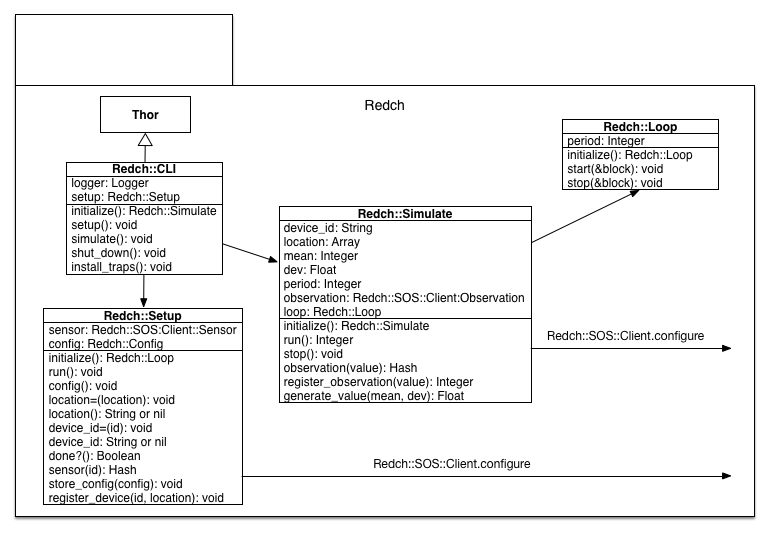
\includegraphics[width=\textwidth]{cli_class_diagram}
	\caption{CLI class diagram}
	\label{fig:cli_class_diagram}
\end{sidewaysfigure}

\begin{sidewaysfigure}
	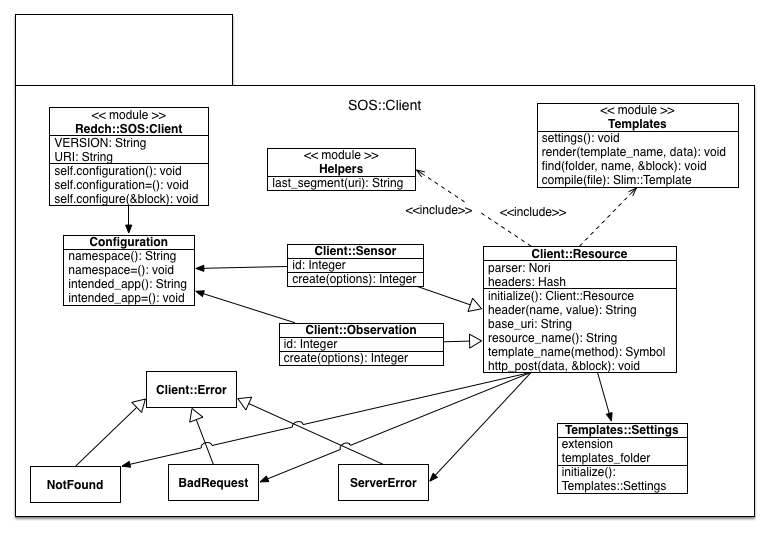
\includegraphics[width=\textwidth]{sos_client_class_diagram}
	\caption{SOS Client class diagram}
	\label{fig:sos_client_class_diagram}
\end{sidewaysfigure}

\subsection{Messaging Queue}

The messaging queue is the central component which drives the data throughout the system and thereby determines the architecture of all other components. A detailed list of most known messaging queue systems has been given in \ref{message_passing}, all of which highly reliable and high-performant. However, usually message queues aren't system bottlenecks but rather message consumers slowed down by database queries or backend systems.

So the choice of an specific message queue depends on the amount of client libraries available, particularly for the languages used in the project, clustering support and the complexity of installation and management. It is also important that the chosen queue has enough high-quality online resources to ease the integration. RabbitMQ, with a rich management web UI and exhaustive documentation including a clustering guide, is the one that best fits our requirements.

This decision has an impact on the design of the data producers and consumers, which must integrate with RabbitMQ using the AMQP protocol. This will be discussed further in following sections.

\subsection{Sensor Observation Service}

Given the CREAF's determination towards the SWE initiative and its involvement in  the open-source GIS community, it is important to make use of the Sensor Observation Service (SOS). To do so, we opt for 52ºNorth SOS 4.0, the leading open-source implementation already integrated by many research institutions throughout the world. In this regard, great efforts are underway to bring latest web standards to the OGC implementations, which may be worth looking into in order to include them in the REDCH project. This is the case of 52ºNorth SOS 4.0. While this project uses its beta version, the final version was released less than three months before this writing.

As fully discussed in \ref{interoperability}, SOS provides the level of interoperability the project requires. This specification structures the service with a core and four extensions: Transactional, Enhanced operations, Result handling and bindings. Together, all extensions provide CRUD functionality for sensors, observations and results.

With regard to the bindings, only SOAP and KVP are defined in the specification. In addition, 52ºNorth SOS 4.0 implements a RESTful binding as part of the bindings extension which our SOS client will use. By choosing this binding, we aim to build a lightweight and stateless service client that can run in a resource-constrained sensor device.

Additionally, 52ºNorth SOS also provides an administrator GUI that enables changing the settings, de/activation of encodings and bindings as well as queries and clearance of stored data.

In order to integrate with RabbitMQ, a component that handles the data delivery to the messaging queue must be developed and included in the SOS. Once the observation has been stored in the database, this component publishes a message with the observation into the queue. Its logical architecture is shown in figure \ref{fig:amqp_extension}.

\begin{figure}[p]
	\centering
	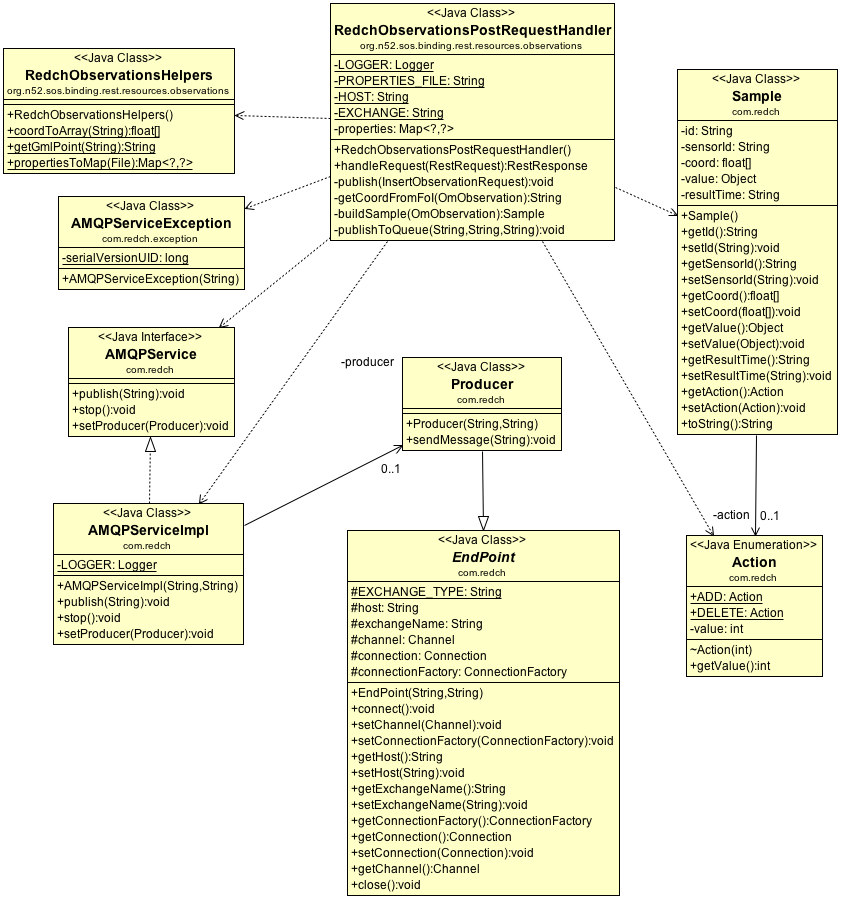
\includegraphics[width=\textwidth]{amqp_extension}
	\caption{SOS AMQP extension}
	\label{fig:amqp_extension}
\end{figure}

\subsection{Database}

52ºNorth's implementation uses Hibernate and Hibernate Spatial persistence framework to allow changing the underlying database management system and database model, which currently supports PostgreSQL/PostGIs, Oracle/Oracle spatial, My\-SQL and SQL Server DBMSs. Although we have chosen PostgreSQL, the GIS industry standard, REDCH may benefit from the integration of some sort of NoSQL solution.

The system is characterised by an ever-growing data set with small data units. That is, the system is write-intensive and I/O-bound. Given this features, in a real-world scenario REDCH may take advantage of massive NoSQL scalability and higher performance. Furthermore, in this project the impact of relaxed consistency may not be as high as in other systems where high reliability is required.

However, time constraints do not allow further exploration of this possibility since this would require that the whole relational schema migrate to a non-relational one. In addition, this prototype will only deal with a limited number of sensors for testing purposes.

\subsection{Web Application}

The web application has two differentiated parts: the application's backend and the Single-Page Application (SPA). While the former pushes AMQP messages received from the queue to the SPA, the latter converts this information into a data visualization. Both components are tied together through a simple Sinatra Application.

\begin{figure}[h]
	\centering
	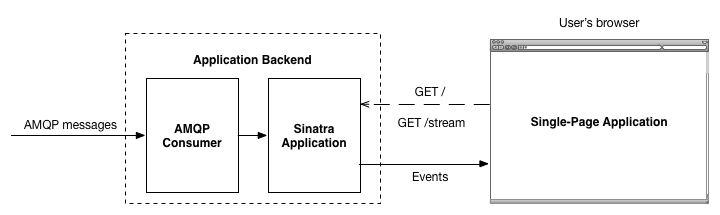
\includegraphics[width=\textwidth]{webapp_logic_view}
	\caption{Web Application's Logic View}
	\label{fig:webapp_logic_view}
\end{figure}

\subsubsection{Backend}

The backend uses the amqp gem. A feature-rich asynchronous RabbitMQ client which is built on top of EventMachine, the most popular event-driven I/O and concurrency library in Ruby. This library implements the Reactor pattern \cite{reactor}, the event handling pattern that constitutes the core of Python's Twisted or Node.js.

Once a message is received, the backend forwards it to each open streaming connection using the HTML5 Server Sent Events API, explained in \ref{web_real_time}. Therefore, concurrency is essential for the performance of the backend which, once again, is provided through EventMachine.

SSE has been chosen over WebSockets as the data delivery mechanism because of its much easier implementation and lesser impact on the underlying infrastructure. Moreover, since the data flows only from the backend to the browser, half-duplex one-way communication is enough.

Sinatra is a Web application framework and Domain Specific Language (DSL) that enables quick creation of web applications in Ruby. In contrast with other frameworks, such as Ruby on Rails, Sinatra does not include a complex ORM nor follows the MVC pattern, focusing instead on being small and flexible.

The Sinatra Application exposes just two endpoints: \texttt{GET /} and \texttt{GET /stream}. The former is used to download the whole SPA, whereas the latter allows for an SSE streaming connection to be opened.

The class diagram of the whole backend is as follows.

\begin{figure}[h]
	\centering
	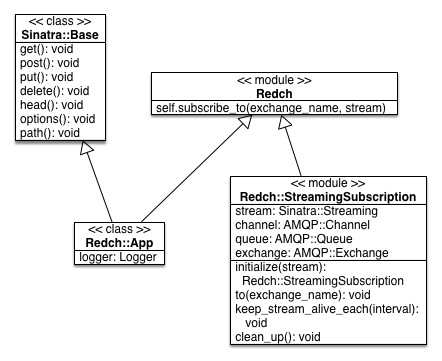
\includegraphics[scale=.7]{backend_class_diagram}
	\caption{Backend class diagram}
	\label{fig:backend_class_diagram}
\end{figure}

\subsubsection{Single Page Application}

The SPA downloads all necessary source codes ---HTML, JS and CSS--- at the first request and renders the data visualization, empty at this point. Then, an HTTP streaming connection is opened  through which the SSE events are sent. Then, the data visualization is continuously rendered with every event containing an observation by using the D3.js JS library. The state of the application is handled through Backbone.js which structures it as a collection of observation models.

The SPA consists of four different components: the HTML template, the data visualization, the data handling and the SSE client.

\begin{figure}[h]
	\centering
	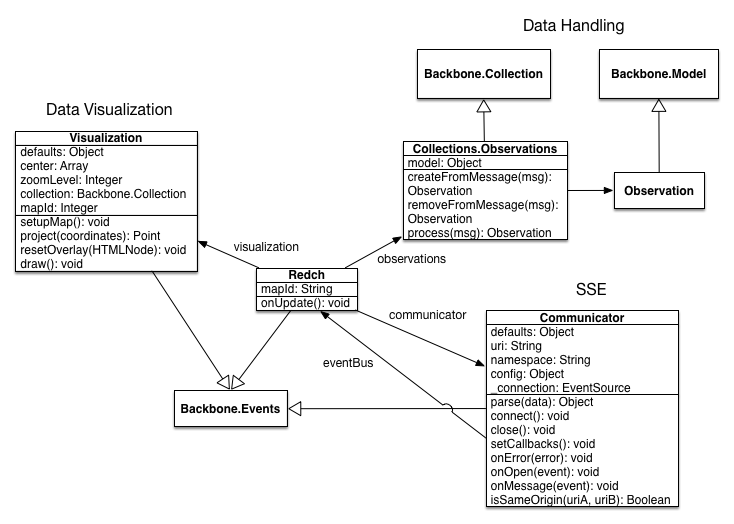
\includegraphics[scale=.55]{spa_class_diagram}
	\caption{SPA class diagram}
	\label{fig:spa_class_diagram}
\end{figure}

The single HTML file acts as the template for the application and contains the references to all of its assets: css files, web fonts, and JS libraries. Among these assets, there are the JS and tiles that Mabpox -- the interactive maps JS library used -- loads.

The data visualization sets up the map and renders circles placed at the exact location where the observation took place, each one corresponding to a different observation. These circles convey the observation's electrical power with the filling color ranging from yellow to red following a linear function.

All SPA pieces work in a fully evented fashion. Whenever a SSE message is received, the \texttt{Communicator} publishes the event into the \texttt{eventBus} and the observations collection, which is subscribed to said event, process it. When the collection triggers an add, remove or change event the visualization gets updated with new, changed or deleted circles depending on the information contained in the collection at that point.

\section{Sequence Diagrams}

This section aims to depict the lifetime of an observation as it goes through all the aforementioned steps from the sensor up until it is visualized in the SPA, thereby giving an overall view of the system's functioning.

\begin{sidewaysfigure}
	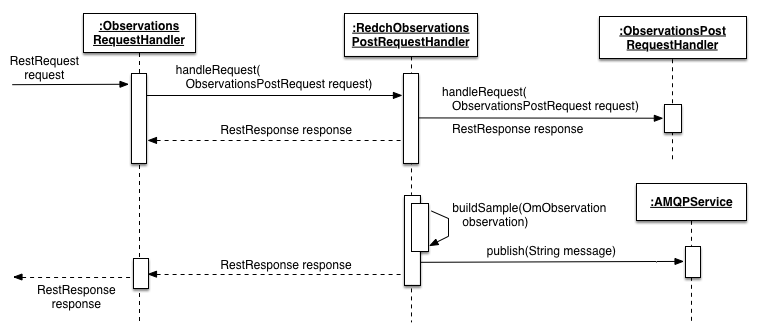
\includegraphics[width=\textwidth]{insert_observation_design_seq}
	\caption{Sequence Diagram - Insert Observation}
	\label{fig:insert_observation_design_seq}
\end{sidewaysfigure}

\begin{figure}[h]
	\centering
	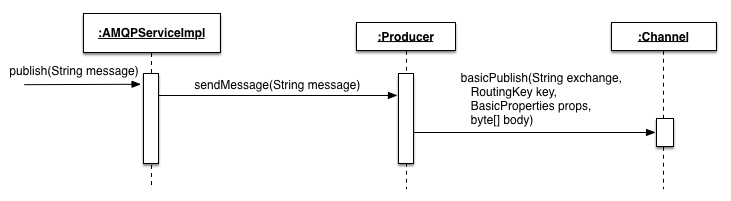
\includegraphics[width=\textwidth]{amqp_service_design_seq}
	\caption{Sequence Diagram - Publish Observation}
	\label{fig:amqp_service_design_seq}
\end{figure}

\begin{figure}[h]
	\centering
	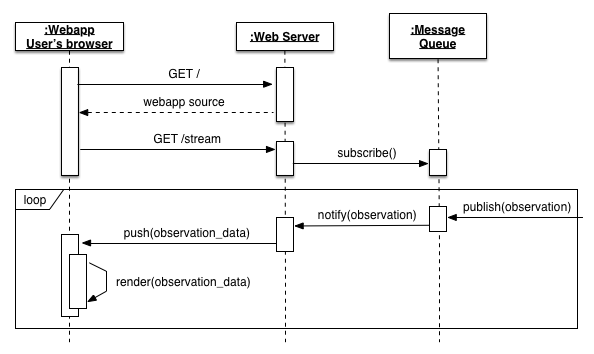
\includegraphics[scale=.7]{browse_data_design_seq}
	\caption{Sequence Diagram - Browse Data}
	\label{fig:browse_data_design_seq}
\end{figure}

%% This is an example first chapter.  You should put chapter/appendix that you
%% write into a separate file, and add a line \include{yourfilename} to
%% main.tex, where `yourfilename.tex' is the name of the chapter/appendix file.
%% You can process specific files by typing their names in at the 
%% \files=
%% prompt when you run the file main.tex through LaTeX.
\chapter{Implementation}

\section{Development environment set-up}

The development of this project comprehends a set of diverse tools that aim to ease this process allowing to focus on the particularities of this project rather than on repetitive and common tasks. What follows is the description and reasons that led to their choice.

\paragraph{Terminal emulator} iTerm2 has been used as the terminal emulator throughout the project to execute many tools used in this project. From the compilation of the customized SOS to the execution of the simulator's CLI. Its rich features such as search, split panes, tabs, 256 colors or OS native notifications support make it a good replacement for the Mac OS X terminal.

\paragraph{Editors} Given the diversity of languages used in the project different editors have been used in its development. An static language like Java requires the use of a full-featured Integrated Development Environment (IDE) like Eclipse, which provides integration with major frameworks and tools. As for the dynamic languages of the project, Ruby and JavaScript, Sublime Text 2 has been chosen as the main editor, sometimes replaced with Vim. Both are lightweight editors with a rich environment of plugins and focused on the efficiency of the developer.

\paragraph{Version Control System} Is essential for the sake of the project to store it in a Version Control System (CVS). Its whole codebase as well as this document are kept in multiple Git repositories. In addition, Github has been chosen as the as the code hosting service due to its focus on collaboration and its considerable popularity in the open-source community.
	
\paragraph{Virtual Machines} Virtual Machines (VM) have been mainly used for the use of multiple sensor simulators at once. A tool such as Vagrant has dramatically improved the use of such systems by providing means to easily configure lightweight and portable development environments. It has become as simple as describing the VM in a file and boot it typing \texttt{vagrant up} in the terminal. The same configuration file can boot the same VM in any other host OS with vagrant installed.

\begin{listing}[h]
\begin{minted}[
frame=lines,
framesep=2mm,
baselinestretch=1.2,
fontsize=\footnotesize,
linenos
] {ruby}
VAGRANTFILE_API_VERSION = '2'
Vagrant.configure(VAGRANTFILE_API_VERSION) do |config|
  config.vm.box = 'sensor-precise32'
  config.vm.provision :shell, path: 'provisioning.sh'

  config.vm.define :sensor0 do |s0|
    s0.vm.host_name = 'sensor0'
    s0.vm.network :private_network, ip: '192.168.0.2'
  end

  config.vm.define :sensor1 do |s1|
    s1.vm.host_name = 'sensor1'
    s1.vm.network :private_network, ip: '192.168.0.3'
  end

  config.vm.define :sensor2 do |s2|
    s2.vm.host_name = 'sensor2'
    s2.vm.network :private_network, ip: '192.168.0.4'
  end
end
\end{minted}
\caption{Example of a Vagrantfile specifying three sensor simulator's VM}
\end{listing}

\paragraph{Secure Shell} the Secure Shell (SSH) has provided to be essential for the development of the project. Once the aforementioned VMs are running the easiest and fastest way to manage them is using ssh through the terminal. Likewise, ssh is the only way to remotely manage the production servers.
%% This is an example first chapter.  You should put chapter/appendix that you
%% write into a separate file, and add a line \include{yourfilename} to
%% main.tex, where `yourfilename.tex' is the name of the chapter/appendix file.
%% You can process specific files by typing their names in at the 
%% \files=
%% prompt when you run the file main.tex through LaTeX.
\chapter{Infrastructure}

This chapter aims to describe the tools and processes involved in the infrastructure setup, from local development environment to the set of production servers running the Redch. Firstly, it explains the infrastructure setup and secondly, describes the provisioning and deployment processes.

\section{Amazon AWS setup}

Amazon Web Services (AWS) is a cloud computing platform that offers a collection of remote computing services ranging from computing and storage to networking services such as DNS, among others. AWS is a world-wide leader of Infrastructure-as-a-Service (IaaS) providers with numerous companies like Spotify, Heroku, Airbnb, Foursquare, Github, Reddit or Mapbox relying on them.

The whole infrastructure of the system is made up of EC2 instances, virtual servers in Amazon's cloud. They all run a custom Amazon Machine Image (AMI) built from a raw Ubuntu 12.04 LTS with all needed dependencies ---Puppet and Ruby 2.0.0--- installed. As a result, any new instance booted up with this custom AMI is ready to be provisioned. Starting and stopping machines, as well as configuring their firewall rules is managed through the AWS Management Console, a web UI.

One of the major benefits Redch can take advantage of is Amazon's Auto Scaling. This service allows to scale the capacity of the EC2 instances up and down according to a set of predefined conditions. A load balancer, for instance, can automatically spawn app servers during demand spikes and shut them down during low demand periods. Redch can get the most out of it by exploiting the fact that solar panels don't produce energy at night, thereby minimizing costs. Likewise, less computing power is required under windless conditions.

Although it would be desirable to keep a provider-independent infrastructure, Amazon RDS has been chosen as database server which makes it easier to set up, operate and scale a relational database. Furthermore, it provides automated backups, Multi-AZ replication and monitoring metrics. It has support for MySQL, Oracle, SQL Server and PostrgeSQL, all the DBMSs supported by 52ºNorth SOS, being the latter the one it uses by default. However, the PostrgeSQL support is still in beta version due to its recent release in November of 2013.

The final production environment consists of the four servers shown in \ref{fig:infrastructure}. Three EC2 micro instances plus a RDS micro instance. Amazon's free tier includes both services at no cost within the first year. Therefore, EC2 micro instances are limited to 1 low-capacity throttled CPU with 627MB of RAM \footnote{AWS Micro Instances Documentation: \url{http://docs.aws.amazon.com/AWSEC2/latest/UserGuide/concepts_micro_instances.html}}. All three EC2 instances are attached to an 8GB Elastic Block Storage (EBS), which are storage volumes with built-in redundancy. These volumes host the filesystem of their attached EC2 instances.

\begin{sidewaysfigure}
  \centering
  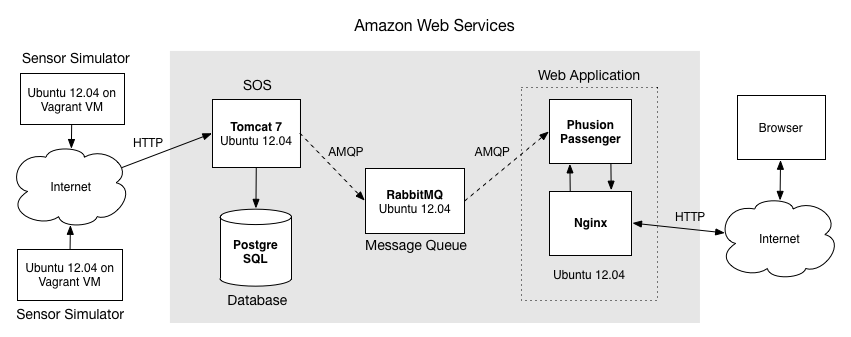
\includegraphics[width=\textwidth]{infrastructure}
  \caption{Production's infrastructure diagram}
  \label{fig:infrastructure}
\end{sidewaysfigure}

Ubuntu 12-04 LTS has been chosen as the OS of all three servers due to its stability and security as well as the inherent benefits of a Linux OS. With regard to the database, Amazon RDS abstract away from the particularities of the underlying hardware by providing the database access as a service.

\section{Provisioning}

Once the software is developed, the underlying infrastructure must be configured to host each of the system components. This process, which involves creating directories and installing packages, may be error-prone when done manually. Besides, the process may need to be repeated several times whenever new servers are set up. Although writing down the build-out process may help, whoever reads that documentation may not be able to figure out the current state of the configuration.

Server automation frameworks formalize systems administration treating infrastructure as code. As a result, infrastructure configuration can be tested and repeated, automating away repetitive tasks while systems administrators focus on architecting and tunning services.

Puppet, among other solutions such as Chef, enables server configuration automation. It automates server provisioning by formalizing its configuration into manifests. Puppet's manifests are text files that contain statements written in a declarative DSL that allows the desired state of the infrastructure to be defined. Once these configurations are deployed, Puppet automatically installs the necessary packages and ensures that the machine’s files and services match the desired state.

\begin{listing}[h]
\begin{minted}[
frame=lines,
framesep=2mm,
baselinestretch=1.2,
fontsize=\footnotesize,
linenos
] {puppet}
package { 'apache2':
  provider => 'apt',
  ensure   => 'installed'
}

service { 'apache2':
  ensure => 'running'
}
\end{minted}
\caption{Example of Puppet's manifest file}
\label{fig:puppet}
\end{listing}

Puppet is mature and widely used and besides having an open source version, there are lots of learning materials available online.

Prior provisioning, any server must have Puppet installed which comes packaged as a ruby gem and therefore, also requires a MRI Ruby interpreter. Puppet can also be installed with any system package manager, but doing so will likely install previous releases missing features and bug fixes.

Puppet enables provision machines by either applying the configuration directly or compiling into a catalog and distributing it to the target system via a client-server paradigm.

\subsection*{Production Software}

Most of the software used in the development environment is also used in production. This is the case of SOS, for instance, where both Tomcat 7 and PostgreSQL have been chosen to run also in production. However, the production web application stack differs from the one used in development. Nginx plus Passenger has been chosen over Thin, the server included in Sinatra for development purposes.

Passenger is a mature and feature-rich application server widely used in many production scenarios. Therefore, is easy to find learning materials and support on the internet. Nginx on the other hand, is a high-performance web server and load balancer that can handle high concurrency.

Placed in front of the application server, Nginx acts as a reverse-proxy. It deals with all incoming requests serving static files efficiently and passing them to the application layer. Passenger then processes the requests and returns a response.

\section{Deployment}

Once the configuration is applied, the target server is up and ready. Next, the code release must be transferred to the production environment to make the application available for use.

Capistrano is a remote multi-server automation tool that enables the execution of arbitrary tasks on remote servers over SSH. It aims to allow reliable deployment of web applications to any number of machines simultaneously. All of its features enforce sane development workflows.

The general configuration of the application is set in the \texttt{deploy.rb} file. Then, each particular stage overrides it in its own file. By following this convention, Capistrano infers the environment names and enables tasks to be run on each of them as in \ref{fig:capistrano}.

\begin{listing}[h]
\begin{minted}[
frame=lines,
framesep=2mm,
baselinestretch=1.2,
fontsize=\footnotesize,
linenos
] {ruby}
set :application, 'redch'
set :repo_url, 'git://github.com/sauloperez/redch-webapp.git'
set :ssh_options, {
  forward_agent: true
}

ask :branch, proc { `git rev-parse --abbrev-ref HEAD`.chomp }

set :deploy_to, '/var/redch'
set :use_sudo, false
set :deploy_via, :copy
set :copy_strategy, :export

SSHKit.config.command_map[:rake]  = "bundle exec rake"

after 'deploy:publishing', 'nginx:restart'
after 'deploy:publishing', 'passenger:restart'
\end{minted}
\caption{Capistrano's deployment definition}
\label{fig:deploy.rb}
\end{listing}

\begin{figure}[h]
  \texttt{\$ cap staging deploy}\\
  \texttt{...}\\
  \texttt{\$ cap production deploy:rollback}\\
  \caption{Execution of commands in different environments}
  \label{fig:capistrano}
\end{figure}

The configuration can be tailored to fit the needs of the project by writing extra tasks. Capistrano provides the \textit{deploy} and \textit{rollback} flows that invoke several hooks for the developer to hook up custom tasks into the flow. In line 16 of listing \ref{fig:deploy.rb} Nginx is restarted right after the release has been published and before the deploy's leftovers are cleaned up.

Therefore, some custom Capistrano tasks have been developed to ease the execution of common operations such as starting and stopping tomcat. The listing \ref{fig:cap_nginx} illustrates Nginx-related tasks used in the web application's deployment. As Capistrano essentially executes commands in a remote server, these custom tasks can written to target any specific purposes such as listing servers' uptimes, checking their load, etc.

\begin{listing}[h]
\begin{minted}[
frame=lines,
framesep=2mm,
baselinestretch=1.2,
fontsize=\footnotesize,
linenos
] {ruby}
namespace :nginx do
  desc 'Start nginx'
  task :start do
    on roles(:app), in: :sequence, wait: 5 do
      sudo 'start nginx'
    end
  end

  desc 'Stop nginx'
  task :stop do
    on roles(:app), in: :sequence, wait: 5 do
      sudo 'stop nginx'
    end
  end

  desc 'Restart nginx'
  task :restart do
    on roles(:app), in: :sequence, wait: 5 do
      sudo 'restart nginx'
    end
  end
end
\end{minted}
\caption{Content of \texttt{lib/capistrano/tasks/nginx.cap}}
\label{fig:cap_nginx}
\end{listing}

%% This is an example first chapter.  You should put chapter/appendix that you
%% write into a separate file, and add a line \include{yourfilename} to
%% main.tex, where `yourfilename.tex' is the name of the chapter/appendix file.
%% You can process specific files by typing their names in at the 
%% \files=
%% prompt when you run the file main.tex through LaTeX.
\chapter{Infrastructure}

This chapter aims to describe the tools and processes involved in the infrastructure setup. From local development environment to the set of production servers running the Redch. Firstly, it explains the infrastructure setup and secondly, it describes the provisioning and deployment processes.

\section{Amazon AWS setup}

Amazon Web Services (AWS) is a cloud computing platform. It is a collection of remote computing services ranging from computing services, with the well-known Amazon EC2, and storage services, with Amazon S3, to networking services such as DNS among others. AWS is a world-wide leader of Infrastructure-as-a-Service (IaaS) providers. A number of high-profile websites like Spotify, Airbnb, Foursquare Github and Mapbox rely on Amazon Web Services.

The whole infrastructure is compound by EC2 instances, virtual servers in Amazon's cloud. They all run a custom Amazon Machine Image (AMI) built from a raw Ubuntu 12.04 LTS AMI installing all needed dependencies: Puppet and Ruby 2.0.0. As a result any new instance booted up with this custom AMI is ready the be provisioned. Starting and stopping machines, as well as configuring their firewall rules is managed through the AWS Management Console, a web UI.

One of the major benefits Redch can take advantage of is Auto Scaling. It allows to scale the number of EC2 instances up and down according to a set of predefined conditions. The load balancer, for instance, can automatically spawn app servers based on load. Redch can get the most out of it exploiting the fact that solar panels don't produce energy at night, so no requests from those sensors will be received during night. This allows to reduce the computing power to bare minimum. (wind mills?)

As for the database server, although it is desirable to keep the infrastructure provider-independent, we choose Amazon RDS. It makes easier to set up, operate, and scale a relational database. Furthermore, it provides automated backups, Multi-AZ replication and monitoring metrics. It has support for MySQL, Oracle, SQL Server and PostregSQL, the DBMS 52North SOS uses. However, due to its recent release in November of 2013 it is still in beta version.

\section{Provisioning}

Once the software is developed the underlying infrastructure must be configured to run each of the system components. This process, that involves creating directories and installing packages, may be error-prone when done manually. Besides, it may need to be repeated next time we have to set up another server. Even though, writing down the build-out process may help, whoever reads that documentation can't figure out the current state of the configuration.

Puppet, among other solutions such as Chef, is a software that enables server configuration automation. It automates server provisioning by formalizing its configuration into manifests. Puppet's manifests are text files that contain statements written in a declarative domain-specific language (DSL) that allows to define the desired state of the infrastructure. Once these configurations are deployed, Puppet automatically installs the necessary packages and ensures that the machine’s files and services match the desired state.

Moreover, Puppet is a mature and widely used product with open source version and lots of tutorials and other learning materials are available online.

Server automation frameworks formalize systems administration treating infrastructure as code. As a result, infrastructure's configuration can be tested and repeated, automating away repetitive tasks while systems administrators focus on architecting and tunning services.

First of all any server to be provisioned must have puppet installed, which comes packaged as a ruby gem. Therefore, Puppet requires an MRI Ruby interpreter. As of this writing, the current stable release is the 3.4.3 which supports 2.0.x ruby versions. Although Puppet can be installed with any system package manager, it will likely install previous releases missing features and bug fixes.

Puppet allows to provision a machines by login into them through ssh and running


%% This is an example first chapter.  You should put chapter/appendix that you
%% write into a separate file, and add a line \include{yourfilename} to
%% main.tex, where `yourfilename.tex' is the name of the chapter/appendix file.
%% You can process specific files by typing their names in at the 
%% \files=
%% prompt when you run the file main.tex through LaTeX.
\chapter{Project Management}

\section{Planning}

The project started with full-time dedication in September 2013 and was planned to be finished by December 2nd, 2013. The first steps were to study its feasibility in terms of technology, to outline the vision and specify the requirements with CREAF. Next steps included the design and implementation of the identified major components of the solution. It would end with the infrastructure setup, testing and the writing of the current document.

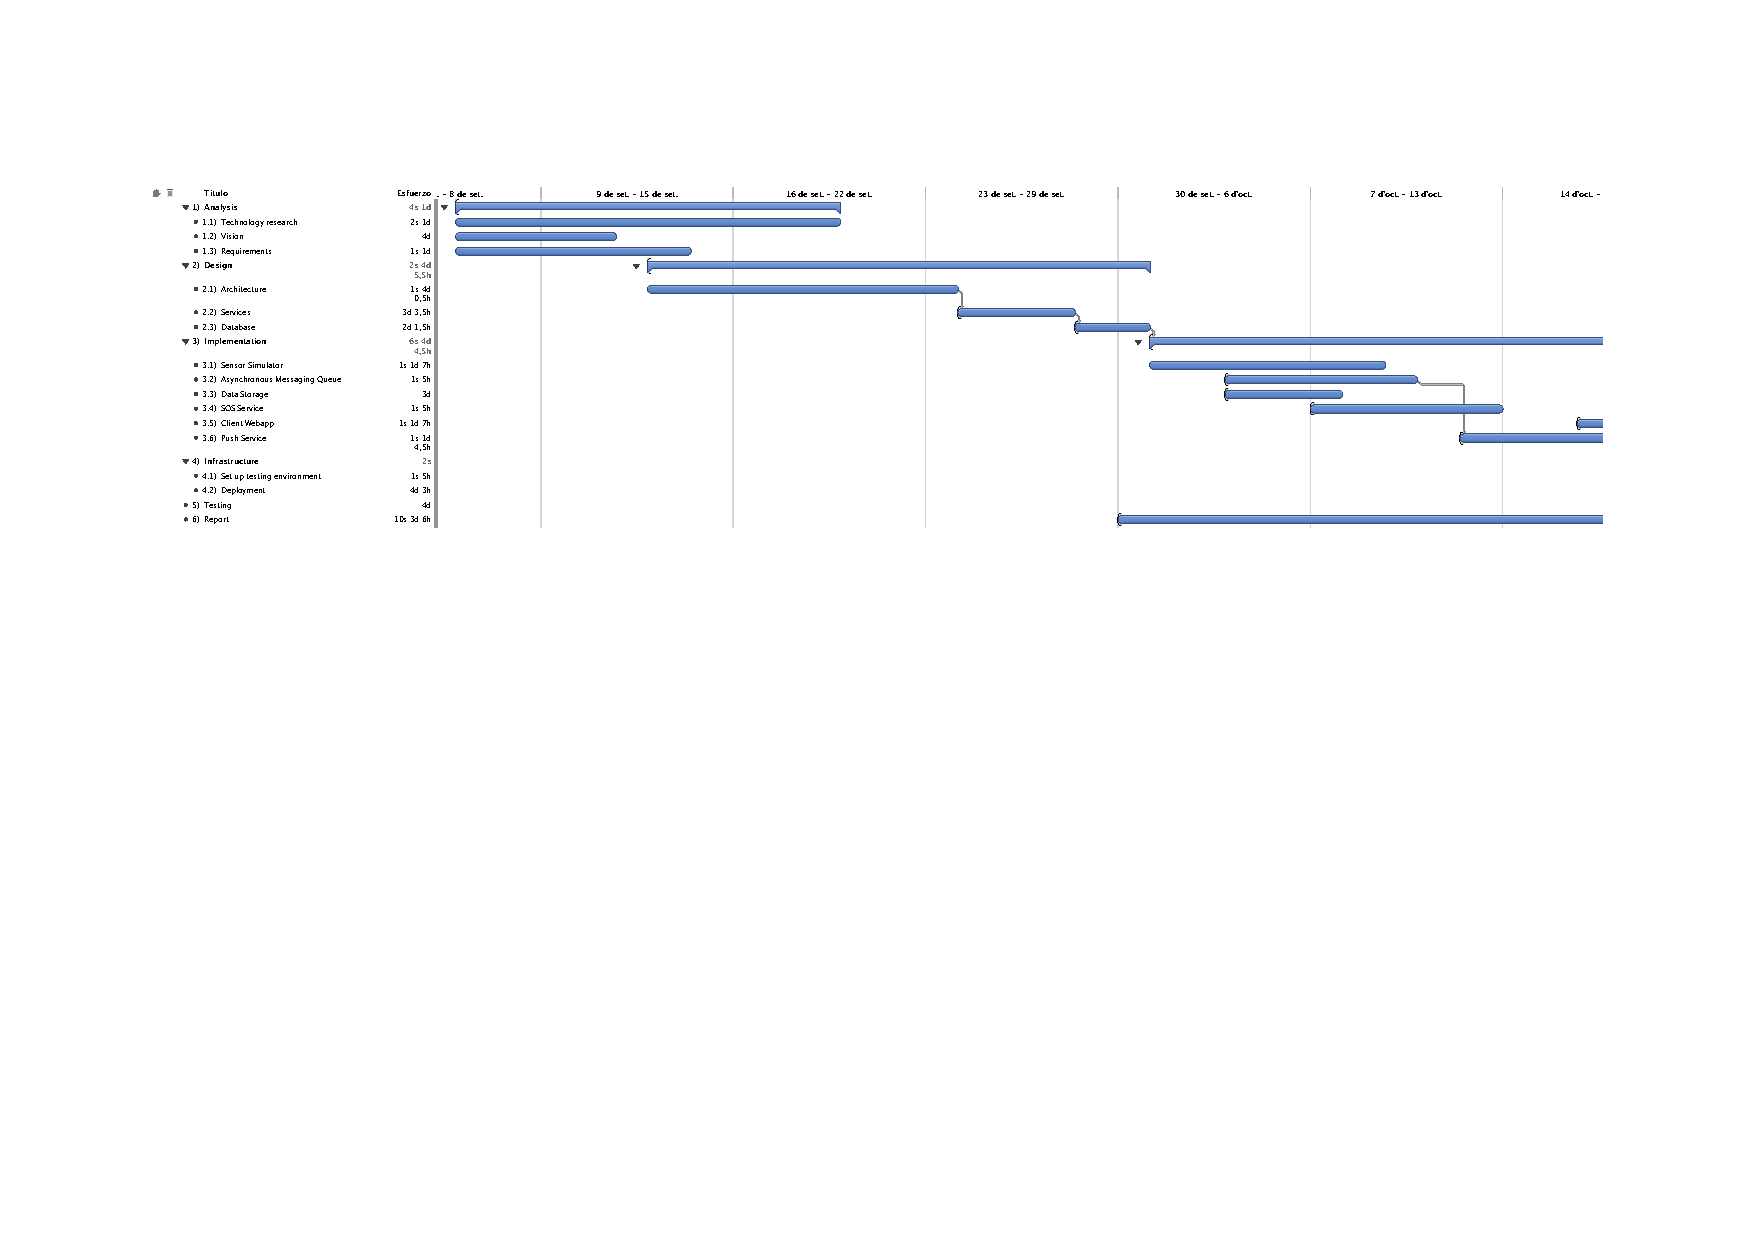
\includepdf[landscape=true, pages={1-2}]{initial_planning}

\section{Cost}

The human resources involved in the project must be considered in order to forecast the costs of the project. These are an analyst who will be in charge of the Analysis and Design, a Developer who will implement the design and a System administrator who will set up the infrastructure.

Regarding the infrastructure, as it relies only on AWS free tier it will not incur in any cost. Therefore, considering these human resources and the initial planning, the overall cost is $15250\euro{}$, as detailed below.

\begin{table}[H]
    \centering
    \begin{tabular}{|l|c|c|r|}
    \hline
    \textbf{Resource}  & \textbf{Cost/Hour}  & \textbf{Hours}  & \textbf{Cost} \\ \hline
    Analyst            & 40\euro{}/h         & 200             & 8000\euro{}   \\ \hline
    Developer          & 25\euro{}/h         & 250             & 6250\euro{}   \\ \hline
    SysAdmin           & 20\euro{}/h         & 50              & 1000\euro{}    \\ \hline
    \textbf{Overall}   &                     &                 & \textbf{15250\euro{}} \\ \hline
    \end{tabular}
    \caption{Budget}
    \label{tab:budget}
\end{table}

Besides the time spent on the different stages of the development, additional time must be considered in order to write the current document. To that end, 90 additional hours plus the $200h + 250h + 45h = 495h$ invested by these human resources must be allocated, totalling $495h + 100h = 600h$.

\section{Execution}

Unfortunately, initial planning has suffered a few setbacks during its execution. It was first delayed at the beginning of December due to my need of finding a job and the time I spent working on a technical test required for a job offer. The major delay was caused by the impact the full-time job had in the dedication time, causing the project to be nearly stopped for several weeks. Although working on it occasionally, it was not until allocating 2 hours every day and full-time dedication on weekends that the project took effectively off. As a consequence, the planning for the remaining tasks was defined as follows.

Regarding the cost, AWS free tier provided not to be enough to fulfil the needs of the required infrastructure. Using three servers exceeded the maximum of 750 hours of EC2 micro instance usage. Thus, the overall cost has been 20.27\$ so far, missing the cost of June 2014.

Moreover, another delay was encountered while executing this final planning. A disproportionately large Amazon AWS bill was received for what seemed to be either an attack on the system or a billing error. This required infrastructure to be shut down until the issue was resolved. Although having some impact, fortunately it didn't excessively affect planning.

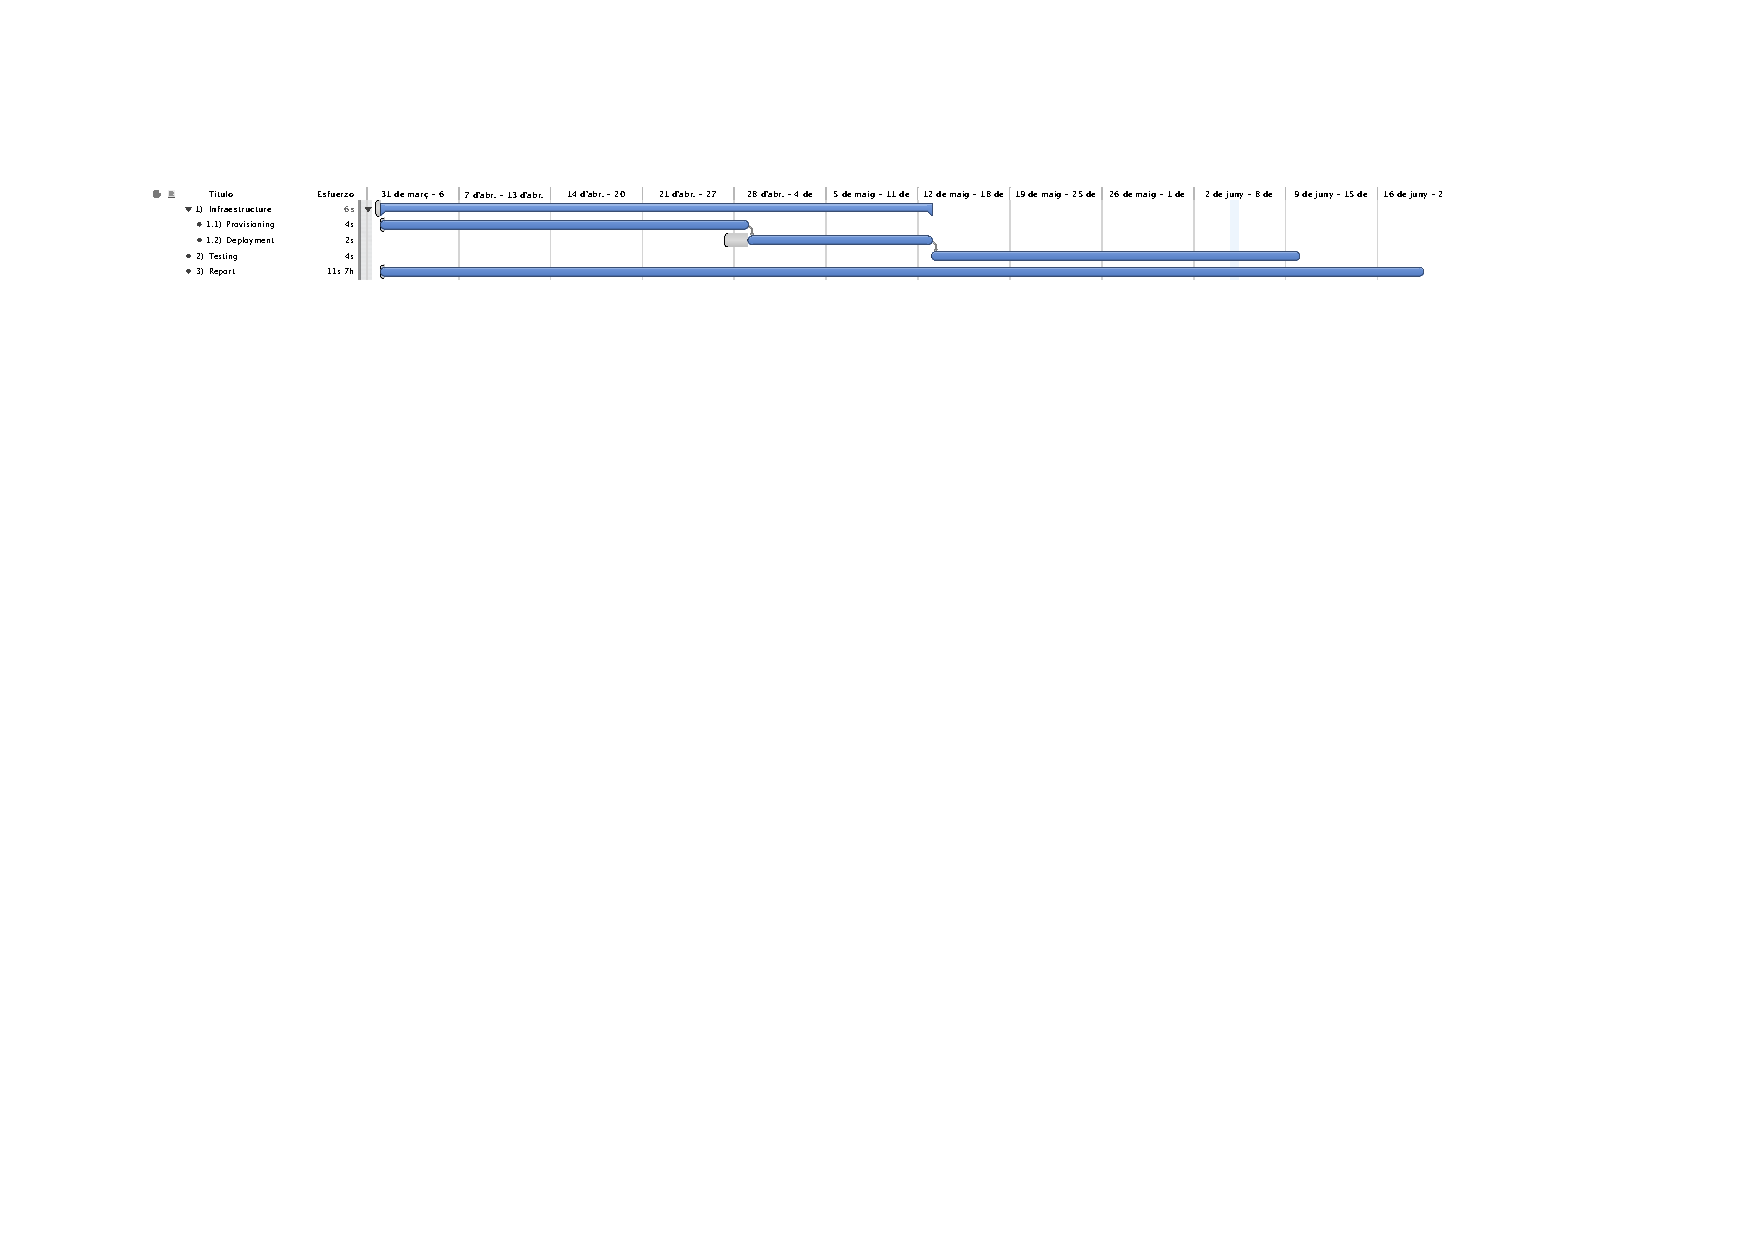
\includepdf[landscape=true, pages={1-2}]{final_planning}
%% This is an example first chapter.  You should put chapter/appendix that you
%% write into a separate file, and add a line \include{yourfilename} to
%% main.tex, where `yourfilename.tex' is the name of the chapter/appendix file.
%% You can process specific files by typing their names in at the 
%% \files=
%% prompt when you run the file main.tex through LaTeX.
\chapter{Conclusions}

\section{Conclusions}

The number of open-source software and modern web technologies used in this MS Thesis have proven to be a viable solution for building IT infrastructure for public research centers. Specifically, these technologies have been combined together to build a distributed system as a proof-of-concept for REDCH, a larger initiative -- named after this thesis -- that aims to provide a valuable insight into the actual production of renewable energies at a small scale in Catalonia.

The introduction presents the motivations behind this initiative of the CREAF and outlines the main goals of this project.

Next, a thorough analysis defines the boundaries of this thesis by providing its scope and requirements. This is detailed further in Chapter 3 with a formal specification of the use cases and the whole conceptual model around the measurement and processing of observations.

Then, Chapter 4 details the findings of the deep research process that had been carried out 
to later support the design decisions taken in Chapter 5. These chapters are particularly relevant due to the fact the chosen technologies are the basis for its further development.

Chapters 6 and 7 provide insight into the implementation and the infrastructure the system runs on. Particular attention is given to the automation of common processes such as provisioning, deployment and maintenance tasks, which provide reliability and confidence to the system's managers. Then, the evaluation of the resulting system in terms of performance is described in Chapter 8.

In spite of the difficulties that determining the scope of the product entailed, the final delimitation we came up with together with CREAF has proven to be adequate. It has been enough to explore each individual part of the project and demonstrate their potential. Specifically, although being rather simple the web application shows how a data visualization can be enriched with a full-featured application. As for the future sensors, the development of the simulator has allowed to better understand the challenges and requirements their design may involve.

On the other hand, the key point of using a messaging queue has been a very successful decision, in that has enabled a loosely coupled and scalable architecture that allows both ends of the queue, the SOS and the web application, to evolve independently. But as downside, this has brought some complexity that affects the resilience of the system. Implementing a more robust redundancy-based resilience mechanism would have improved the overall quality of the system.

As for the infrastructure, the complexity of setting the servers up surpassed the initial estimation causing a great impact on the time invested for that matter. While running the services in a development environment is often very easy, there are numerous variables involved when it comes to a production environment. Furthermore, it was the least-known of the fields involved in the project and the one that required the deepest understanding of the architecture. This led us to the conclusions that being the infrastructure critical for the proper functioning of the system, much attention has to be paid to the administration of the system. Otherwise, its impact on cost will increase as it evolves.

Regarding the methodology, the outcome of the iterative development is a clean and maintainable codebase. A first iteration laid out each component and allowed to get the insight upon which the second iteration improved them so as to be up and ready.

Finally, all the goals of the project have been successfully achieved and all the requirements in Chapter 2 were met. We are able to simulate sensors with a command line interface and the observations are stored, processed and displayed in real time.

\section{Further Work}

Considering the current state of the product, we identify some unresolved issues and steps that would be worth exploring in further research.

From the point of view of the implementation, there are a couple of aspects of the current architecture that would be interesting to investigate. First, given the event-driven nature of the web application's  back-end, it may be worth replacing its implementation with Node.js. Its non-blocking I/O design that claims to maximize throughput and efficiency, makes it suitable for scalable networking applications. This seems to be a natural fit the features of this project and may even surpass the EventMachine's high performance. However, it has not been possible due to the time constraints considering our total lack of awareness of this platform.

Regarding the messaging queue, given that RabbitMQ's messages acknowledgement is not used may be beneficial to implement messaging with Redis instead. It is essentially a very high-performance key/value store for structured data that brings many other features such as pub/sub capabilities. This, however, doesn't include message acknowledgement for the sake of performance. Replacing RabbitMQ with Redis would enable to implement retrieval of latest observations once a new browser connection is established, feature that isn't currently supported. Nevertheless, Redis pub/sub simplicity compared to RabbitMQ queue features may impact on future decisions as the system's usage grows.

From the infrastructure perspective, it may be beneficial at the early stages of the project to lean towards a Platfor-as-a-service (PaaS) hosting rather than the current IaaS. As a result, it would require far less systems administration knowledge and it would simplify deployments even more, but this comes at the expense of higher cost and less control over the product. In any case, this a possibility that is worth studying.

Finally, as next step of the project the system's poor performance must be addressed by switching to more reliable and powerful servers. Regarding the sensors, the physical sensor devices must be developed taking the ideas brought in the research as the starting point. Besides, the SOS must be upgraded to the 52ºNorth SOS 4.0 final release.

After that, it would be recommended to start using the system with a small subset of real users while the ideas exposed above are considered prior to a public release. Meanwhile it would be valuable to look for the involvement of public institutions, other research centers and specially the Open Geospatial Consortium so as to ensure the success of the project. Once a steady number of active users use the system, it would be the time to explore using AWS Auto Scaling. At a much later stage, the big data set would benefit from migrating to a NoSQL database, thereby increasing the scalability of the system.

\appendix
\chapter{Tables}

\begin{table}
\caption{Armadillos}
\label{arm:table}
\begin{center}
\begin{tabular}{||l|l||}\hline
Armadillos & are \\\hline
our	   & friends \\\hline
\end{tabular}
\end{center}
\end{table}

\clearpage
\newpage

%% This defines the bibliography file (main.bib) and the bibliography style.
%% If you want to create a bibliography file by hand, change the contents of
%% this file to a `thebibliography' environment.  For more information 
%% see section 4.3 of the LaTeX manual.
\begin{singlespace}
\begingroup
\raggedright
\bibliography{main}
\bibliographystyle{plain}
\endgroup
\end{singlespace}

\end{document}

